%%%%%%%%%%%%%%%%%%%%%%%%%%%%%%%%%%%%%%%%%
% University/School Laboratory Report
% LaTeX Template
% Version 3.1 (25/3/14)
%
% This template has been downloaded from:
% http://www.LaTeXTemplates.com
%
% Original author:
% Linux and Unix Users Group at Virginia Tech Wiki 
% (https://vtluug.org/wiki/Example_LaTeX_chem_lab_report)
%
% License:
% CC BY-NC-SA 3.0 (http://creativecommons.org/licenses/by-nc-sa/3.0/)
%
%%%%%%%%%%%%%%%%%%%%%%%%%%%%%%%%%%%%%%%%%

%----------------------------------------------------------------------------------------
%	PACKAGES AND DOCUMENT CONFIGURATIONS
%----------------------------------------------------------------------------------------

\documentclass{article}

\usepackage[version=3]{mhchem} % Package for chemical equation typesetting
\usepackage{siunitx} % Provides the \SI{}{} and \si{} command for typesetting SI units
\usepackage{graphicx} % Required for the inclusion of images
\usepackage{natbib} % Required to change bibliography style to APA
\usepackage{amsmath} % Required for some math elements 
\usepackage{gensymb}
\usepackage{textcomp}
\usepackage{eucal}
\usepackage{amsmath}
\usepackage{listings}
\usepackage{color} %red, green, blue, yellow, cyan, magenta, black, white
\usepackage{verbatim}
\usepackage{courier}
\definecolor{mygreen}{RGB}{28,172,0} % color values Red, Green, Blue
\definecolor{mylilas}{RGB}{170,55,241}


\setlength\parindent{0pt} % Removes all indentation from paragraphs

\renewcommand{\labelenumi}{\alph{enumi}.} % Make numbering in the enumerate environment by letter rather than number (e.g. section 6)

%\usepackage{times} % Uncomment to use the Times New Roman font

%----------------------------------------------------------------------------------------
%	DOCUMENT INFORMATION
%----------------------------------------------------------------------------------------

\title{Homework 1 \\ Project Report \\ Camera Calibration} % Title

\author{\textsc{Fnu Karan} \\ NetID: kx361} % Author name

\date{\today} % Date for the report

\begin{document}

\maketitle % Insert the title, author and date

\begin{center}
\begin{tabular}{l r}
Date Performed: & February 19, 2017 \\ % Date the experiment was performed
Instructor: & Professor Gerig % Instructor/supervisor
\end{tabular}
\end{center}

% If you wish to include an abstract, uncomment the lines below
% \begin{abstract}
% Abstract text
% \end{abstract}

%----------------------------------------------------------------------------------------
%	SECTION 1
%----------------------------------------------------------------------------------------

\section{Objective}

The objective is to calibrate a camera for a fixed focal length using two orthogonal checkerboard planes, and to find intrinsic and extrinsic parameters.

%If you want something in the center use this:
%\begin{center}\ce{2 Mg + O2 -> 2 MgO}\end{center}

% If you have more than one objective, uncomment the below:
%\begin{description}
%\item[First Objective] \hfill \\
%Objective 1 text
%\item[Second Objective] \hfill \\
%Objective 2 text
%\end{description}

%For a subsection use this:
%\subsection{Definitions}
%\label{definitions}
%\begin{description}
%\item[Stoichiometry]
%The relationship between the relative quantities of substances taking part in a reaction or forming a compound, typically a ratio of whole integers.
%\item[Atomic mass]
%The mass of an atom of a chemical element expressed in atomic mass units. It is approximately equivalent to the number of protons and neutrons in the atom (the mass number) or to the average number allowing for the relative abundances of different isotopes. 
%\end{description} 
 
%----------------------------------------------------------------------------------------
%	SECTION 2
%----------------------------------------------------------------------------------------

\section{Experimental Procedure}
\subsection{Data Capture}
Two checkerboards are places on a wall corner which is at 90{\degree} as shown in the figure below. The world axes are chosen as: The origin is at the lower end where the two checkerboards meet each other. Y axis points upwards from the origin, X axis is towards the right checkboard from the origin and Z axis is towards the left checkerboard from the origin.
\medskip

\begin{figure}[h]
\begin{center}
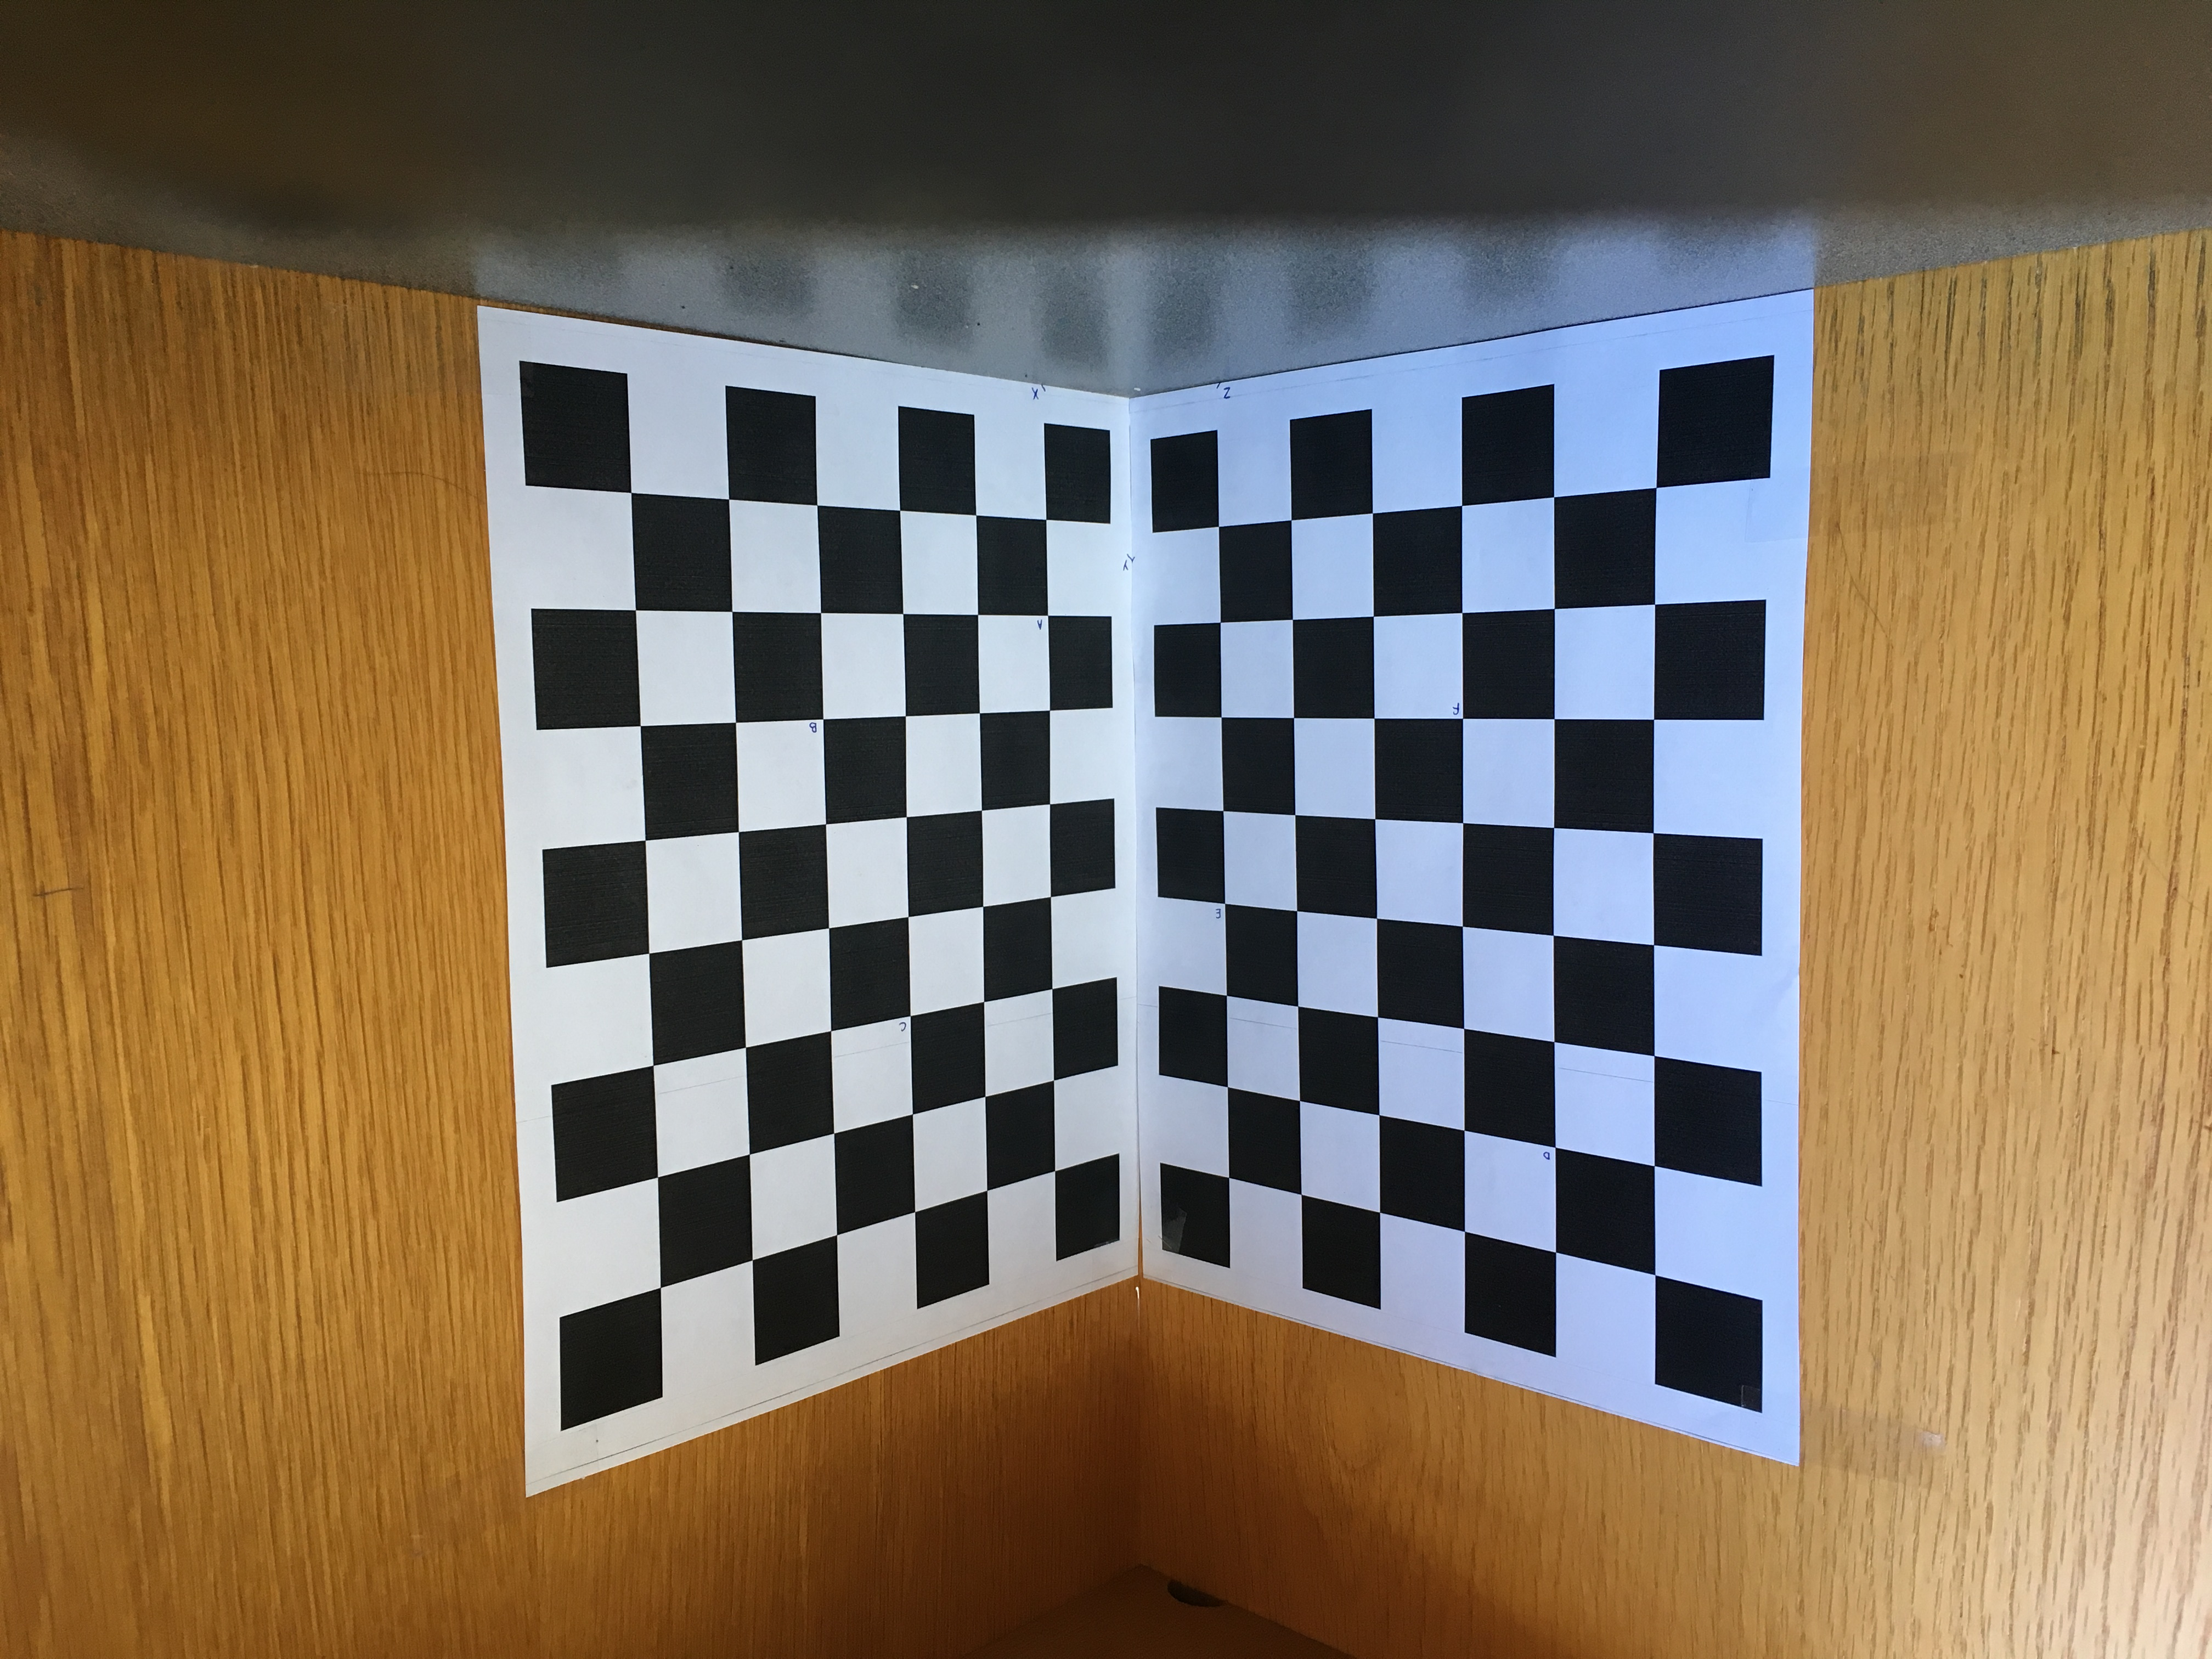
\includegraphics[width=1\textwidth,angle=180]{check_1.jpg} % Include the image placeholder.jpg
\caption{Checkerboard pattern on the corner of the wall and the world frame coordinate axes.}
\end{center}
\end{figure}

The points to be measured are shown with the labels, A to F in the Figure 1. Total six points are chosen, three on one checkerboard and three on the other. All the world frame coordinates are measured in millimeters(mm). Also the distance reorded from camera origin to the world origin is 677 mm. 

\medskip
The picture of the checkerboard pattern is captured using a camera and the coordiantes of these 6 points are measured in the image coordinate frame (with the origin taken at the top left corner of the image). The image resolution is 4032x3024. This step gives us the coordinates of 6 points with their corresponding points in the image. We need to estimate 11 free parameters for the camera calibration so this number of points is sufficient.

\medskip
The camera used was of the phone iPhone 6S. It is 12MP and we can see it in the picture resolution as specified above, and it uses ``Stacked back-illuminated CMOS image sensor'', and its size is 4.80 x 3.60 mm (1/3''). The pixel size is 1.22 $\mu$m. The aperture is f/2.2. The focal length is 4.15 mm. 

\subsection{Estimation of the Calibration Matrix}
Least squares method is used to estimate the calibration matrix. there are 12 homogeneous linear equations in 12 variables, which are the coefficients of the calibration matrix $\CMcal{M}$. Let's denote this system of linear equations as 
\begin{equation}
\CMcal{P}m = 0
\end{equation}

\begin{equation}
m:=\begin{bmatrix} m_1 & m_2 & m_3 \end{bmatrix}^T,
\end{equation}

\medskip
where $m_1, m_2, m_3$ are fist, second and third rows of the matrix $\CMcal{M}$ respectively. m is a 12 x 1 vector, and $\CMcal{P}$ is a 12 x 12 matrix. The problem of least square estimation of $\CMcal{P}$ is defined as

\begin{equation}
min|| \CMcal{P}m ||^2,  \text{ subject to }||m||^2=1.
\end{equation}

\medskip

As it turns out, the solution of above problem is given by the eigenvalue of matrix $\CMcal{P}^T\CMcal{P}$ having the least eigenvalue. The eigenvectors of the matrix $\CMcal{P}^T\CMcal{P}$ can also be computed by performing the singular value decomposition (SVD) of $\CMcal{P}$. The 12 right singluar vectors of $\CMcal{P}$ are also the eigenvectors of $\CMcal{P}^T\CMcal{P}$. The SVD method is used here to get the eigenvector corresponding to the least eigenvalue. This eigenvector is the solution to the above problem. Reorganizing the 12 x 1 vector m in a matrix of 3 x 4 gives us the matrix $\CMcal{M}$. The first three elements of the third row of this matrixx denote one of the three rotation vectors.

\subsection{Computation of Intrinsic and Extrinsic Parameters}
The intrinsic and extrinsic parameters are computed from the calibration matrix $\CMcal{M}$ by using the method given in the book. These methods use the various properties fo the rotation vectors, namely the norm of them being one and the dot product of the two rotation matrices being zero.

\medskip

Once the calibration matrix is estimated, we pick these points again from the checkerboard pattern, and record their coordinates in the world frame. We then transform these points to the image coordinates using the matrix $\CMcal{M}$ that we obtained using the above described method. These image coordinates are then compared to the observed coordinates and finally we give the errors at last. 

%----------------------------------------------------------------------------------------
%	SECTION 3
%----------------------------------------------------------------------------------------

\section{Results}

The estimated calibtation matrix using the above described method obtained is, 
\medskip

\begin{equation}
\CMcal{M} = \begin{bmatrix} 0.00289166 & -0.00016395 & -0.00094185 & -0.94420018 \\
   0.00056440 & -0.00280669 &  0.00065426 & -0.32934464 \\
   0.00000048 & -0.00000006 &  0.00000050 & -0.00045809 \end{bmatrix}
\end{equation}


\begin{center}
\begin{table}
\centering
\begin{tabular}{c|c}
Parameters & Values \\ \hline \hline
$\theta$ &  89.93{\degree} \\
$u_0$ & 1903.371 \\
$v_0$ & 1566.708 \\
$\alpha$ & 3567.708 \\
$\beta$ & 3550.947 \\ \hline
\end{tabular}
\smallskip
\caption{Intrinsic Parameters}
\end{table}
\end{center}

The intrinsic parameters are shown in Table 1. 

The extrinsic parameters consist of the rotation and translation matrix. The rotation matrix is shown below.

\begin{equation}
\CMcal{R} = \begin{bmatrix} -0.07314050     &   -0.99600794  &     -0.05117265 \\
         0.71758403      & -0.01692221    &    -0.69626632 \\
         0.69262083   &    -0.08764595       &  0.71595709 \end{bmatrix}
\end{equation}

\medskip
The translation matrix is estimated as $\rho\CMcal{K}^{-1}b$, where $\CMcal{K}$ is the intrinsic parameter matrix and b is the last column of the matrix $\CMcal{M}$. The obtained translation vector is, 

\begin{equation}
\CMcal{T} = \begin{bmatrix} -89.1718 & 142.7421 &  -649.3070 \end{bmatrix}^T.
\end{equation}


%----------------------------------------------------------------------------------------
%	SECTION 4
%----------------------------------------------------------------------------------------

\section{Discussion}

\subsection{Intrinsic Parameters}
We get $\theta$ almost equal to 90{\degree}, which means that the camera has very little skew, meaning that the X and Y axes in the image frame are almost at 90{\degree} to each other.

\medskip

The image center lies at (2016, 1512). We had ($u_0,v_0$) as (1903.37, 1566.70). The image center does not coincide with $C_0$ and its position is shifted by (112.63, 54.7).

\medskip

$\alpha$ and $\beta$ are equal to \textit{kf} and \textit{lf} repectively. The terms \textit{k} and \textit{l} denote the number of pixels per \textit{mm}, and \textit{f} is the focal length of the lens. 
In our case, focal length is 4.15 mm. The pixel density (pixels per mm) is obtained as,
\begin{equation}
k = \frac{4032}{4.80} = 840
\end{equation}
and
\begin{equation}
l = \frac{3024}{3.60} = 840
\end{equation}
\medskip
Now, we have pixel densities, \textit{k} and \textit{l}. We can find $\alpha$ and $\beta$ as, 
\begin{equation}
\alpha = k*f = 3486
\end{equation}
and
\begin{equation}
\beta = l*f = 3486
\end{equation}
These values of $\alpha$ and $\beta$ are comparable to the ones that we estimated in Table 1. 
\subsection{Extrinsic Parameters}
Three rows of the rotation matrix have their norm equal to 1 and their dot product is almost equal to zero. This is justified very well considering the human error, which cannot be avoided.

\medskip

The translation vector also approximates the real values. We measured the difference between the world origin and the camera origin, which is approximately equal to the $||\CMcal{T}||$. The straight distance was measured as 667 mm and $||\CMcal{T}|| = 670.76$, and these both values are really close. 

\subsection{Image Coordinates Reconstruction}
To revalidate the estimated parameters, we take those 6 points again, and corresponding to these points we also calculate the image coordinates. Along with that we also measure the true image coordinates using MATLAB. The values are shown in Table 2. 

\medskip

The error norm is calculated by subtracting corresponding coordinates and errors along X and Y axes. These errors are then squared and added, and then square root of the resultant is taken to get the error norm. We note that the reconstruction errors are not so big and can be justified given the amount of inherent errors in the measuring process itself.

\begin{center}
\begin{table}
\centering
\begin{tabular}{ l | p{2.8cm} | p{2.8cm} | l}
World Coordinates & Image Coordinates (calculated) & Image Coordinates (measured) & Error norm \\ \hline \hline
(37, 68, 0) & (1909.75, 1124.02) & (1910.64, 1123.23) & 1.192 \\
(121.5, 96, 0)  & (1503.97,1310.25) & (1503.53, 1310.88) & 0.763 \\
(93.5, 181, 0) & (1660.77, 1852.17) & (1660.95, 1851.72) & 0.479\\
(0, 212, 150) & (2832.89, 2089.38) & (2833.45, 2089.04) & 0.653\\
(0, 154.7, 37) & (2237.12,1646.71) & (2236.34, 1647.52) & 1.130\\ 
(0, 98.3, 122) & (2671.01, 1305.22)& (2670.60, 1305.35) & 0.432\\ \hline
\end{tabular}
\smallskip
\caption{Test of Calibration Parameters: Error between measured and estimated image coordinates. All the world coordinates are in mm.}
\end{table}
\end{center}


%----------------------------------------------------------------------------------------
%	SECTION 5
%----------------------------------------------------------------------------------------

\section{MATLAB Code}

\subsection{Important Information about the Code}
The code is done using MATLAB. The real world coordinates and image coordinates were saved in an excel file and then using some features of excel, values of matrix $\CMcal{P}$ were calculated. Once the values of matrix $\CMcal{P}$ are obtained, then we copied it to another excel file from where the matrix $\CMcal{P}$ is read into the MATLAB code. 

\medskip

The intrinsic parameters are stored in the variable named \textit{Intrinsic}, rotation matrix is stored in the variable named \textit{Rotation} and translation matrix is stored in the variable named \textit{Translation}. 

\subsection{The Code}

\lstset{language=Matlab,%
    %basicstyle=\color{red},
    breaklines=true,%
    morekeywords={matlab2tikz},
    keywordstyle=\color{blue},%
    morekeywords=[2]{1}, keywordstyle=[2]{\color{black}},
    identifierstyle=\color{black},%
    stringstyle=\color{mylilas},
    commentstyle=\color{mygreen},%
    showstringspaces=false,%without this there will be a symbol in the places where there is a space
    numbers=left,%
    numberstyle={\tiny \color{black}},% size of the numbers
    numbersep=9pt, % this defines how far the numbers are from the text
    emph=[1]{for,end,break},emphstyle=[1]\color{red}, %some words to emphasise
    %emph=[2]{word1,word2}, emphstyle=[2]{style},    
}

\texttt{\lstinputlisting{script.m}}

\begin{comment}
The accepted value (periodic table) is \SI{24.3}{\gram\per\mole} \cite{Smith:2012qr}. The percentage discrepancy between the accepted value and the result obtained here is 1.3\%. Because only a single measurement was made, it is not possible to calculate an estimated standard deviation.

The most obvious source of experimental uncertainty is the limited precision of the balance. Other potential sources of experimental uncertainty are: the reaction might not be complete; if not enough time was allowed for total oxidation, less than complete oxidation of the magnesium might have, in part, reacted with nitrogen in the air (incorrect reaction); the magnesium oxide might have absorbed water from the air, and thus weigh ``too much." Because the result obtained is close to the accepted value it is possible that some of these experimental uncertainties have fortuitously cancelled one another.

%----------------------------------------------------------------------------------------
%	SECTION 6
%----------------------------------------------------------------------------------------

\section{Answers to Definitions}

\begin{enumerate}
\begin{item}
The \emph{atomic weight of an element} is the relative weight of one of its atoms compared to C-12 with a weight of 12.0000000$\ldots$, hydrogen with a weight of 1.008, to oxygen with a weight of 16.00. Atomic weight is also the average weight of all the atoms of that element as they occur in nature.
\end{item}
\begin{item}
The \emph{units of atomic weight} are two-fold, with an identical numerical value. They are g/mole of atoms (or just g/mol) or amu/atom.
\end{item}
\begin{item}
\emph{Percentage discrepancy} between an accepted (literature) value and an experimental value is
\begin{equation*}
\frac{\mathrm{experimental\;result} - \mathrm{accepted\;result}}{\mathrm{accepted\;result}}
\end{equation*}
\end{item}
\end{enumerate}

%----------------------------------------------------------------------------------------
%	BIBLIOGRAPHY
%----------------------------------------------------------------------------------------


\bibliographystyle{apalike}

\bibliography{sample}

%----------------------------------------------------------------------------------------
\end{comment}

\end{document}